\section{Características das amplitudes (seção 4)}

\subsection{Características calculadas}

Para cada uma das 30 gravações foi usada a série completa de amplitudes do par 20, na ordem original e sem normalização, suavização ou corte. As cinco características são:

{\footnotesize
\begin{longtable}{|>{\centering\arraybackslash}p{2.84cm}|>{\centering\arraybackslash}p{4.57cm}|>{\centering\arraybackslash}p{7.24cm}|}
\caption{Características usadas na análise.}\\
\hline
\textbf{Característica} & \textbf{Cálculo} & \textbf{O que mede / para que serve} \\ \hline
\endfirsthead
\hline
\textbf{Característica} & \textbf{Cálculo} & \textbf{O que mede / para que serve} \\ \hline
\endhead
Média & soma das amplitudes / N & Nível médio do sinal. Depende da posição da pessoa, do ambiente e do ganho do receptor; serve para comparar o nível entre gravações. \\ \hline
Mediana & valor central da série ordenada & Nível típico, pouco sensível a picos isolados. Comparada com a média, indica assimetria e presença de valores extremos. \\ \hline
Desvio padrão & raiz da média dos quadrados dos desvios em relação à média, divisor N (ddof = 0) & Dispersão em torno da média: quanto o sinal varia ao longo da gravação (movimento gera variação). \\ \hline
Pico a pico & máximo - mínimo & Extensão total dos valores; muito sensível a um único valor extremo. \\ \hline
Média das diferenças absolutas & soma de |x(i+1) - x(i)| / (N - 1) & Variação média de um registro para o seguinte (rapidez das mudanças por registro, não por segundo). \\ \hline
\end{longtable}
}

Os resultados das 30 gravações estão em \textbf{caracteristicas\_reais.csv} e na Tabela A1 (Anexo).

\subsection{Gráficos comparativos}

Em cada gráfico, o eixo horizontal tem as cinco atividades, cada cor é um participante (azul s12, vermelho s13, verde s14, iguais nos cinco gráficos) e o símbolo distingue a primeira (círculo) e a segunda (triângulo) gravação: 6 pontos por atividade e 30 por gráfico.

\begin{figure}[H]
    \centering
    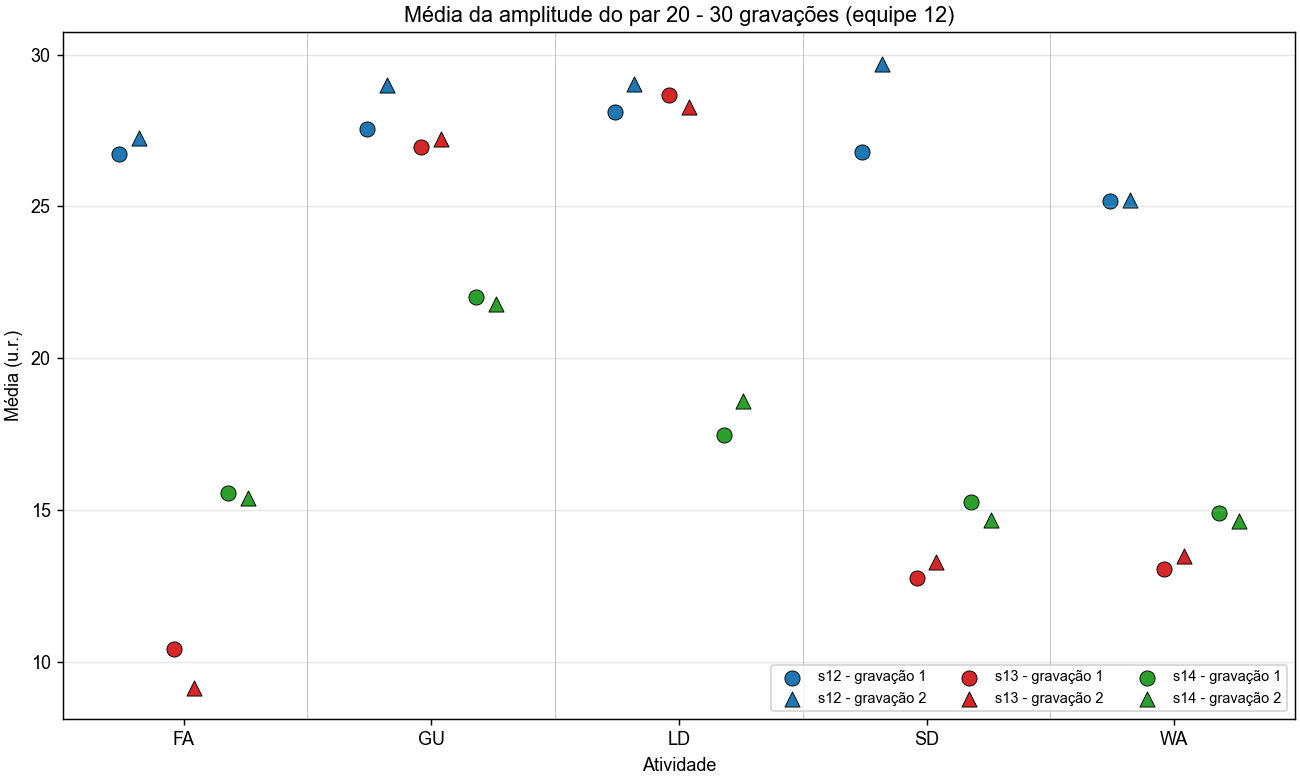
\includegraphics[width=0.85\textwidth,height=19.0cm,keepaspectratio]{Imagens/sec4_grafico1_media.png}
    \caption{Média da amplitude do par 20 nas 30 gravações. (arquivo: figuras/sec4\_grafico1\_media.png)}
    \label{fig:sec4_grafico1_media}
\end{figure}

\begin{figure}[H]
    \centering
    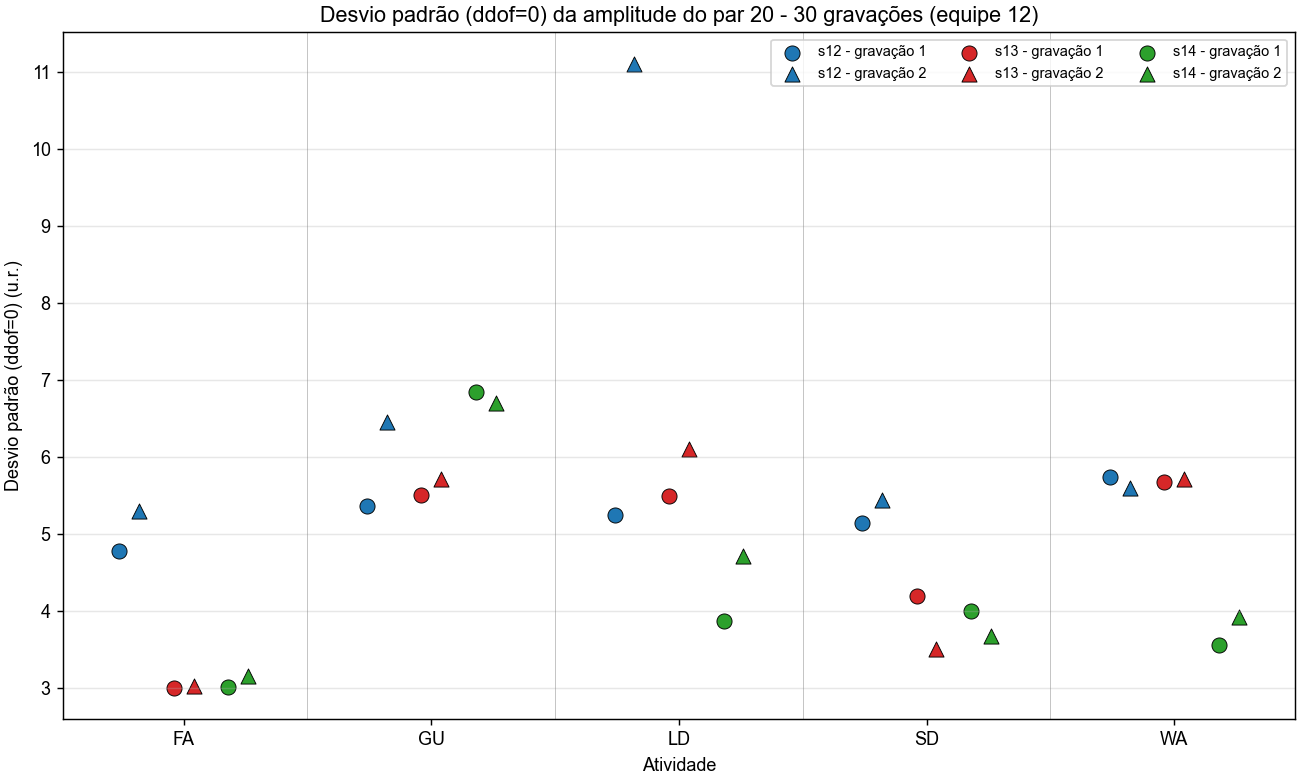
\includegraphics[width=0.85\textwidth,height=19.0cm,keepaspectratio]{Imagens/sec4_grafico3_desvio_padrao.png}
    \caption{Desvio padrão da amplitude do par 20 nas 30 gravações. (arquivo: figuras/sec4\_grafico3\_desvio\_padrao.png)}
    \label{fig:sec4_grafico3_desvio_padrao}
\end{figure}

\begin{figure}[H]
    \centering
    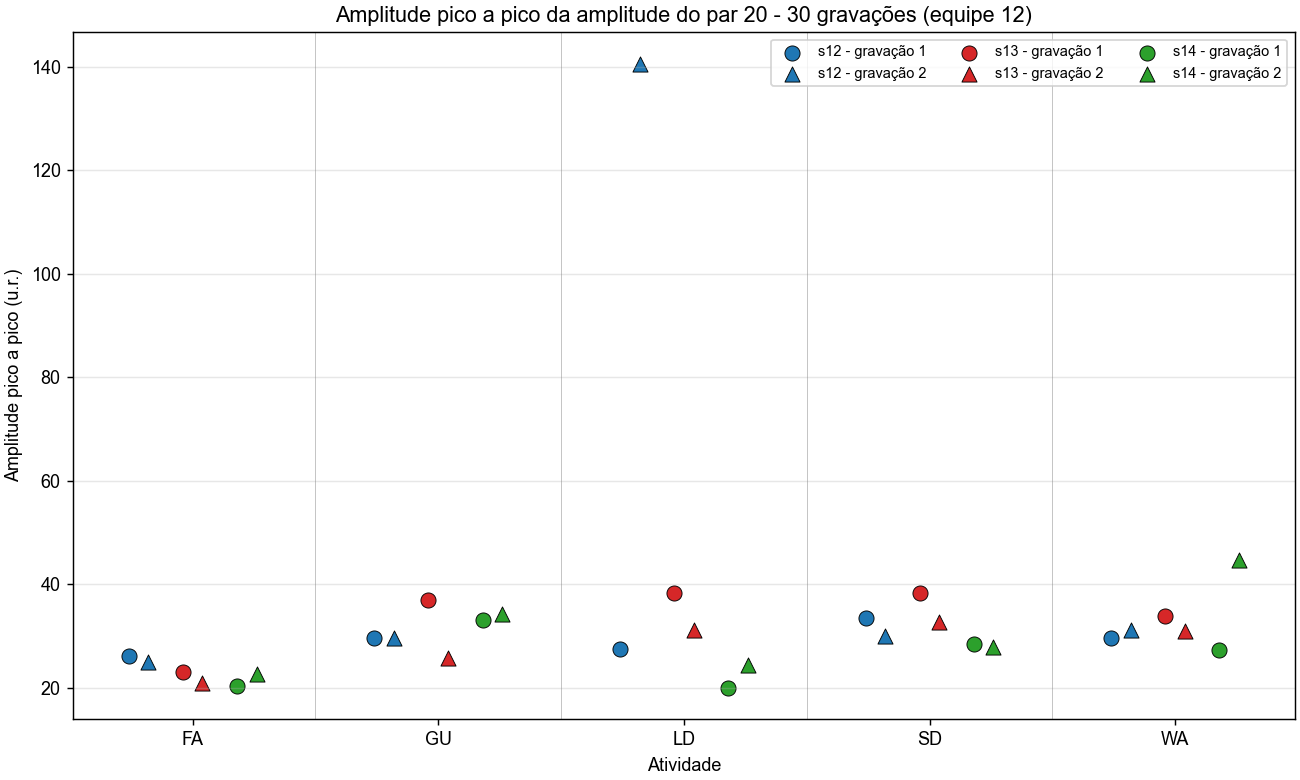
\includegraphics[width=0.85\textwidth,height=19.0cm,keepaspectratio]{Imagens/sec4_grafico4_pico_a_pico.png}
    \caption{Amplitude pico a pico da amplitude do par 20 nas 30 gravações. (arquivo: figuras/sec4\_grafico4\_pico\_a\_pico.png)}
    \label{fig:sec4_grafico4_pico_a_pico}
\end{figure}

\begin{figure}[H]
    \centering
    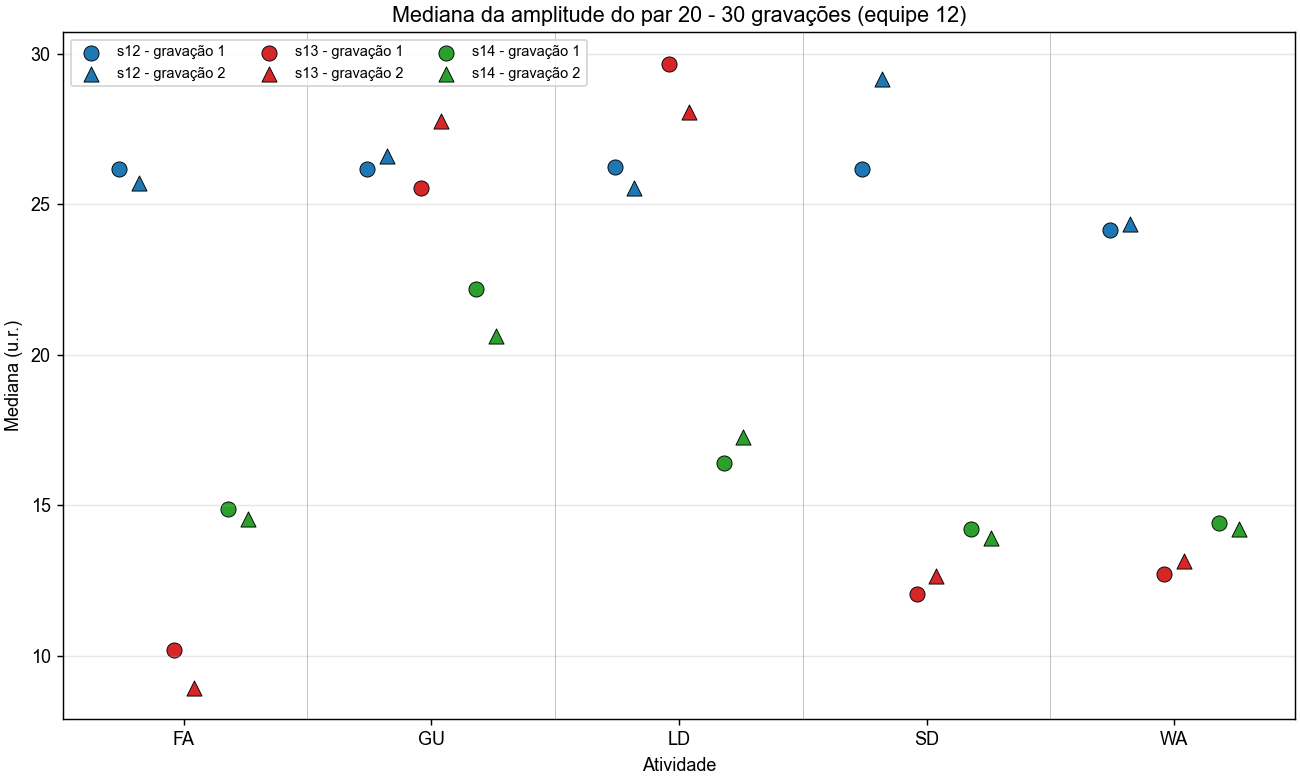
\includegraphics[width=0.85\textwidth,height=19.0cm,keepaspectratio]{Imagens/sec4_grafico2_mediana.png}
    \caption{Mediana da amplitude do par 20 nas 30 gravações. (arquivo: figuras/sec4\_grafico2\_mediana.png)}
    \label{fig:sec4_grafico2_mediana}
\end{figure}

\begin{figure}[H]
    \centering
    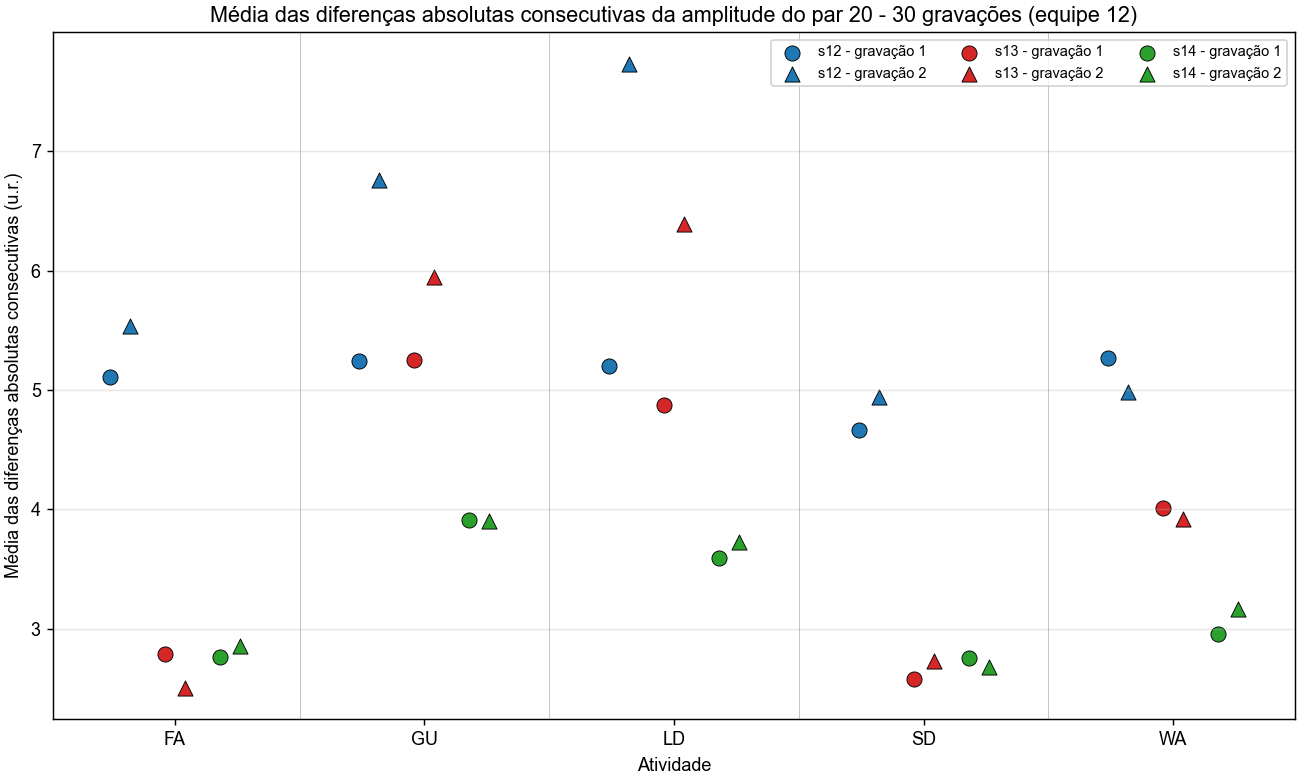
\includegraphics[width=0.85\textwidth,height=19.0cm,keepaspectratio]{Imagens/sec4_grafico5_media_diferencas_absolutas.png}
    \caption{Média das diferenças absolutas entre registros consecutivos da amplitude do par 20 nas 30 gravações. (arquivo: figuras/sec4\_grafico5\_media\_diferencas\_absolutas.png)}
    \label{fig:sec4_grafico5_media_diferencas_absolutas}
\end{figure}

\subsection{Interpretação}

\textbf{1. Duas gravações da mesma pessoa e atividade.} Na maioria dos casos as duas gravações têm características semelhantes. Exemplos: s14/FA, média 15,59 e 15,42, desvio 3,01 e 3,17; s13/WA, média 13,08 e 13,52, desvio 5,68 e 5,71 (Figuras 6 e 7). As exceções são: \textbf{s12/LD}, em que a gravação 2 tem desvio 11,11 contra 5,25, pico a pico 140,63 contra 27,51 e diferença média 7,74 contra 5,20, por causa de picos de até 157 nos registros $\sim$1-250 (visíveis na figura de comparação da dupla s12\_LD, seção 6), enquanto as médias ficam próximas (28,11 e 29,04); \textbf{s12/SD}, com médias 26,80 e 29,70; e \textbf{s14/WA}, com pico a pico 27,26 e 44,69 apesar de desvios parecidos (3,56 e 3,92) - ou seja, um único valor extremo altera o pico a pico sem mudar a dispersão geral.

\textbf{2. Pessoas diferentes, mesma atividade.} Há diferenças acentuadas entre participantes, principalmente no nível (Figuras 6 e 9). Em FA, as médias são 26,72-27,25 (s12), 9,18-10,45 (s13) e 15,42-15,59 (s14), sem sobreposição. Em GU e LD, s12 e s13 se sobrepõem (médias entre $\sim$27 e $\sim$29), enquanto s14 fica abaixo ($\sim$22 em GU e $\sim$17,5-18,6 em LD). A média das diferenças absolutas (Figura 10) também separa os participantes: s12 fica entre 4,7 e 7,7, enquanto s14 fica entre 2,7 e 3,9 em todas as atividades.

\textbf{3. Mesma pessoa, atividades diferentes.} Em \textbf{s13} a média é a característica que mais muda (de 9,18 em FA a 28,67 em LD), acompanhada da diferença média (2,51-2,79 em FA e 2,58-2,73 em SD contra 5,25-5,94 em GU e 4,87-6,39 em LD). Em \textbf{s14}, GU se destaca pelo desvio padrão (6,70-6,84 contra 3,01-3,17 em FA) e pela média ($\sim$22 contra 14,7-18,6 nas demais). Em \textbf{s12} as cinco características variam pouco entre atividades (médias de 25,2 a 29,7; desvios de 4,8 a 6,4, exceto a gravação 2 de LD). Uma hipótese para o caso de s13: os nomes dos arquivos são carimbos de tempo Unix, e as gravações de GU e LD (1722281718 a 1722281947) foram feitas cerca de uma hora antes das de FA, SD e WA (1722284702 a 1722286550). A diferença de nível pode, portanto, refletir mudanças do ambiente ou da posição dos equipamentos entre sessões, e não apenas a atividade.

\textbf{4. Sobreposição entre atividades.} Sim, os valores se sobrepõem bastante. Considerando os três participantes juntos, as médias de FA vão de 9,2 a 27,2 e as de SD de 12,8 a 29,7, cobrindo praticamente a mesma faixa; o pico a pico fica entre $\sim$20 e $\sim$45 em todas as atividades (exceto o valor atípico de s12/LD); e o desvio padrão fica entre $\sim$3 e $\sim$7 para todas. Como a diferença entre pessoas é maior que a diferença entre atividades, essas cinco características de um único par não bastam para distinguir as atividades. Essas conclusões se limitam às 30 gravações analisadas, e a separação visual de pontos não demonstra, por si só, que um classificador reconheceria as atividades.

\newpage
